\chapter{Illumination optics}
This chapter provides some concepts of illumination optics used in this thesis. We start explaining the difference between radiometry and photometry.
In particular, we focus on the photometric variables, defining them both in three and two dimensions. The reflection and refraction laws and the phenomenon of total internal reflection are explained. The last paragraph of the chapter gives a brief introduction to Fresnel reflection. 
\section{Radiometric and photometric variables}\label{sec:photometry}
Radiometry is concerned with the measurement of electromagnetic radiation across the entire electromagnetic spectrum. Photometry is the subfield of radiometry that takes into account only the portion of the electromagnetic spectrum corresponding to the visible light, \cite{zalewski1995radiometry}. Radiometry deals with radiometric quantities. An important radiometric quantity  is the radiant flux $\Phi_{\textrm{r}}$ (unit watt, [\textrm{W}]) which is the total energy emitted from a source or received by a target per unit time:
\begin{equation}
\Phi_{\textrm{r}} = \frac{\textrm{d}Q}{\textrm{d}T}\,,
\end{equation}
where $Q$ is the energy and $T$ the time.\\
\indent In illumination optics the measurement of light is given in terms of the impression that it gives on the human eye. Therefore, illumination optics deals with photometric variables. The most important photometric variables are defined as follows using the same notation adopted by Chaves in \cite{chaves2015introduction}. The luminous flux $\Phi$ (unit lumen, [\textrm{lm}]) is defined as the perceived power of light by the human eye.
 The radiant and the luminous flux are related by the luminous efficacy function, unit [\textrm{lm}/\textrm{W}], which tells us how many lumen there are for each Watt of power at a given wavelength.
 The luminous efficacy reaches its maximum  at a wavelength of $555$ $\textrm{nm}$ where it is equal to $683$ $\textrm{lm}/\textrm{W}$.
  We may normalize the luminous efficacy function with its maximum value of $683$.
  This normalized function is the dimensionless luminosity function $\bar{y}(\lambda)$ shown in Figure $\ref{fig:luminosityfunction}$ where $\lambda$ is the wavelength.
\begin{figure}[h]
%\label{fig:luminousfunction}
  \begin{center}
  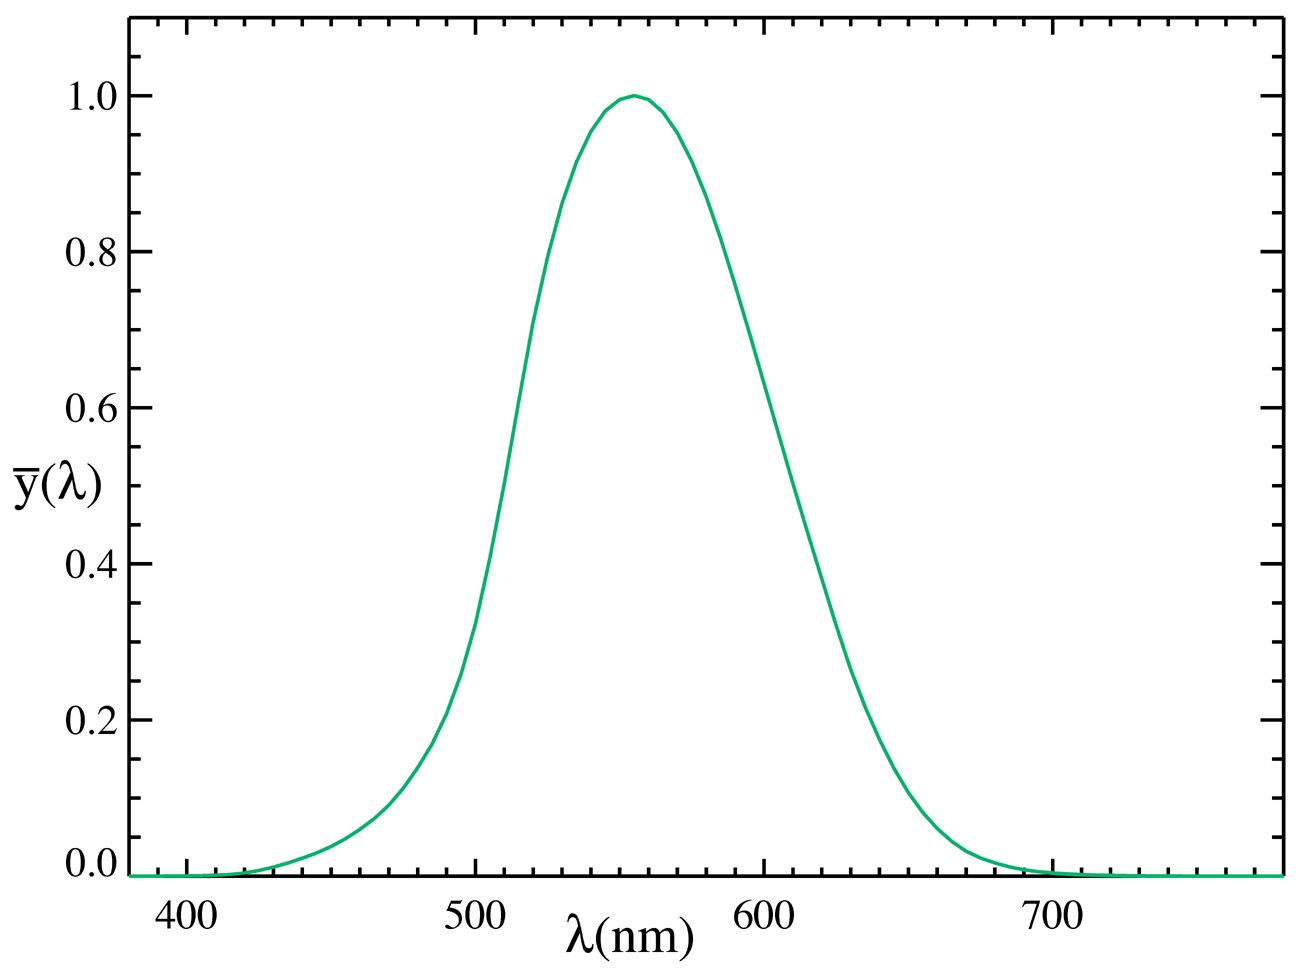
\includegraphics[width=7cm]{CIELuminosity}
  \end{center}
  \caption{Luminosity function $\bar{y}(\lambda)$: relation between the eye's sensitivity and the wavelength of light. The luminosity function is dimensionless, \cite{wiki}.}
  \label{fig:luminosityfunction}
  \end{figure}
\\ \indent The luminous flux corresponding to one Watt of radiation power at any wavelength is given by the product of $683$ $\textrm{lm/W}$ and the luminosity function at the same wavelength,
i.e. $683 \, \bar{y}(\lambda)$. Hence, the total luminous flux $\Phi$ has unit lumen [\textrm{lm}] and it is defined as:
\begin{equation}
\Phi = 683 \int_0^\infty \Psi_\textrm{r}(\lambda) \bar{y}(\lambda)\textrm{d}\lambda
\end{equation}
where $\Psi_\textrm{r}(\lambda)$ is the power in watt per unit wavelength (unit [\textrm{W}/\textrm{m}]). 
\\ \indent A beam of light can be described as a collection of parallel light rays, where a light ray can be interpreted as a path along which the energy travels. 
The luminous flux $\textrm{d}\Phi$ incident on a surface is called illuminance $E$ \big(unit \big[$\textrm{lm}/\textrm{m}^2\big]$\big)
and is defined as:
\begin{equation}
 E=\frac{\textrm{d}\Phi}{\textrm{d}A}\;,
 \end{equation}
 where $\textrm{d}A$ is an infinitesimal area receiving radiation. The density of light emitted by a point source in a given direction is determined by the solid angle. 
The solid angle on a given direction is defined by the infinitesimal surface area $\textrm{d}S$  of a sphere subtended by the radius of that sphere and by the rays emitted by the center on that direction, \cite{arecchi2007field}.  
%The solid angle is indicated with $\Omega$ and the dimensionless unit of solid angles is the steradian $[sr]$, \cite{arecchi2007field}.
 Indicating with $r$ the radius of the sphere, the infinitesimal solid angle $\textrm{d}\Omega$ defined by $\textrm{d}S$  is given by:
\begin{equation}\label{solid_angle}
\textrm{d}\Omega = \frac{\textrm{d}S}{r^2}\,. %= \sin(\theta)\textrm{d}\theta \phi\.
\end{equation}
The solid angle on the entire sphere is $\Omega = 4\pi$, its unit is the steradian $[\textrm{sr}]$  and it is usually defined on a unit sphere .
The luminous intensity $I$ (unit candela (\textrm{cd}), $[\textrm{cd}=\textrm{lm}/\textrm{sr}]$) is defined as the luminous flux $\textrm{d}\Phi$ per solid angle
$\textrm{d}\Omega$ and is given by:
\begin{equation}\label{intensity}
I = \frac{\textrm{d}\Phi}{\textrm{d}\Omega}\;.
\end{equation}
 \begin{figure}[h]
%\label{fig:cup}
  \begin{center}
  \includegraphics[width=6 cm]{SolidAngle}
  \end{center}
  \caption{Solid angle $\textrm{d}\Omega$ in a direction making an angle \myangle $\;$with the normal to the area $\textrm{d}A$.}
  \label{fig:rad}
  \end{figure}The luminance $L$ \big(unit $\big[\textrm{cd} / \textrm{m}^2\big]$\big) is the luminous flux per unit solid angle $\textrm{d}\Omega$ and  per unit projected area $\cos\mbox{\myangle}\,\textrm{d}A$ where \myangle $\,$ is the angle that the normal $\boldsymbol{\nu}$ to the area $\textrm{d}A$ makes with the direction of the solid angle $\textrm{d}\Omega$, as shown in Figure $\ref{fig:rad}$.  $L$  is given by:
\begin{equation}\label{luminance1}
  L=\frac{\textrm{d}\Phi}{\cos\mbox{\myangle}\,\textrm{d}A\textrm{d}\Omega}\,.
\end{equation}
\noindent Note that from ($\ref{intensity}$) and ($\ref{luminance1}$) we can derive a relation between the intensity and the luminance. 
The intensity $I$ emitted by the infinitesimal area $\textrm{d}A$ is given by:
\begin{equation}
I = \frac{\textrm{d}\Phi}{\textrm{d}\Omega}= L(\vect{x},\mbox{\myangle})\cos\mbox{\myangle}\textrm{d}A \,.
\end{equation}
When the luminance is uniform over a finite area $A$, the luminous intensity emitted in the direction \myangle $\,$ is equal to:
\begin{equation}
I(\mbox{\myangle}) = L(\mbox{\myangle}) A \cos\mbox{\myangle}\,.
\end{equation}
Thus, when $L(\vect{x},\mbox{\myangle})$ does not depend on the position and the direction (i.e. $L(\vect{x},\mbox{\myangle})=L$), we obtain Lambert's cosine law:
\begin{equation}
I(\mbox{\myangle}) = I_0\cos\mbox{\myangle}\,.
\end{equation}
where $I_0 = I(0) = LA$. \\
\indent Finally, the \'{e}tendue $U$ (unit $[\textrm{m sr}]$) describes the ability of a source to emitt light or the capability of an optical system to receive light, \cite{zhu2011etendue}.
The quantity $ \textrm{d}U $ is defined as:
\begin{equation}\label{etendue}
\textrm{d}U = n^2 \cos\mbox{\myangle}\textrm{d}A\textrm{d}\Omega.
\end{equation}
where $n$ is the index of refraction of the medium in which the surface $A$ is immersed. In optics the \'{e}tendue is considered to be a volume in phase space  (or an area for two-dimensional systems). This concept will be clarified in Chapter \ref{chap:PS} in which we treat the phase space in more detail.
An important property of the \'{e}tendue is that it is conserved within an optical system in absence of absorption. We now show, using the approach of Chaves in \cite{chaves2015introduction}, 
how conservation of this quantity can be derived.
Consider a light ray emitted from an infinitesimal area $\textrm{d}A_1$ to the area $\textrm{d}A_2$. Suppose that the centers of $\textrm{d}A_1$ and $\textrm{d}A_2$ 
are located at a distance \variabile{d} to each other,  see Figure \ref{fig:etendue_conservation}.
\begin{figure}[h]
 \label{fig:etendue_conservation}
     \begin{center}
     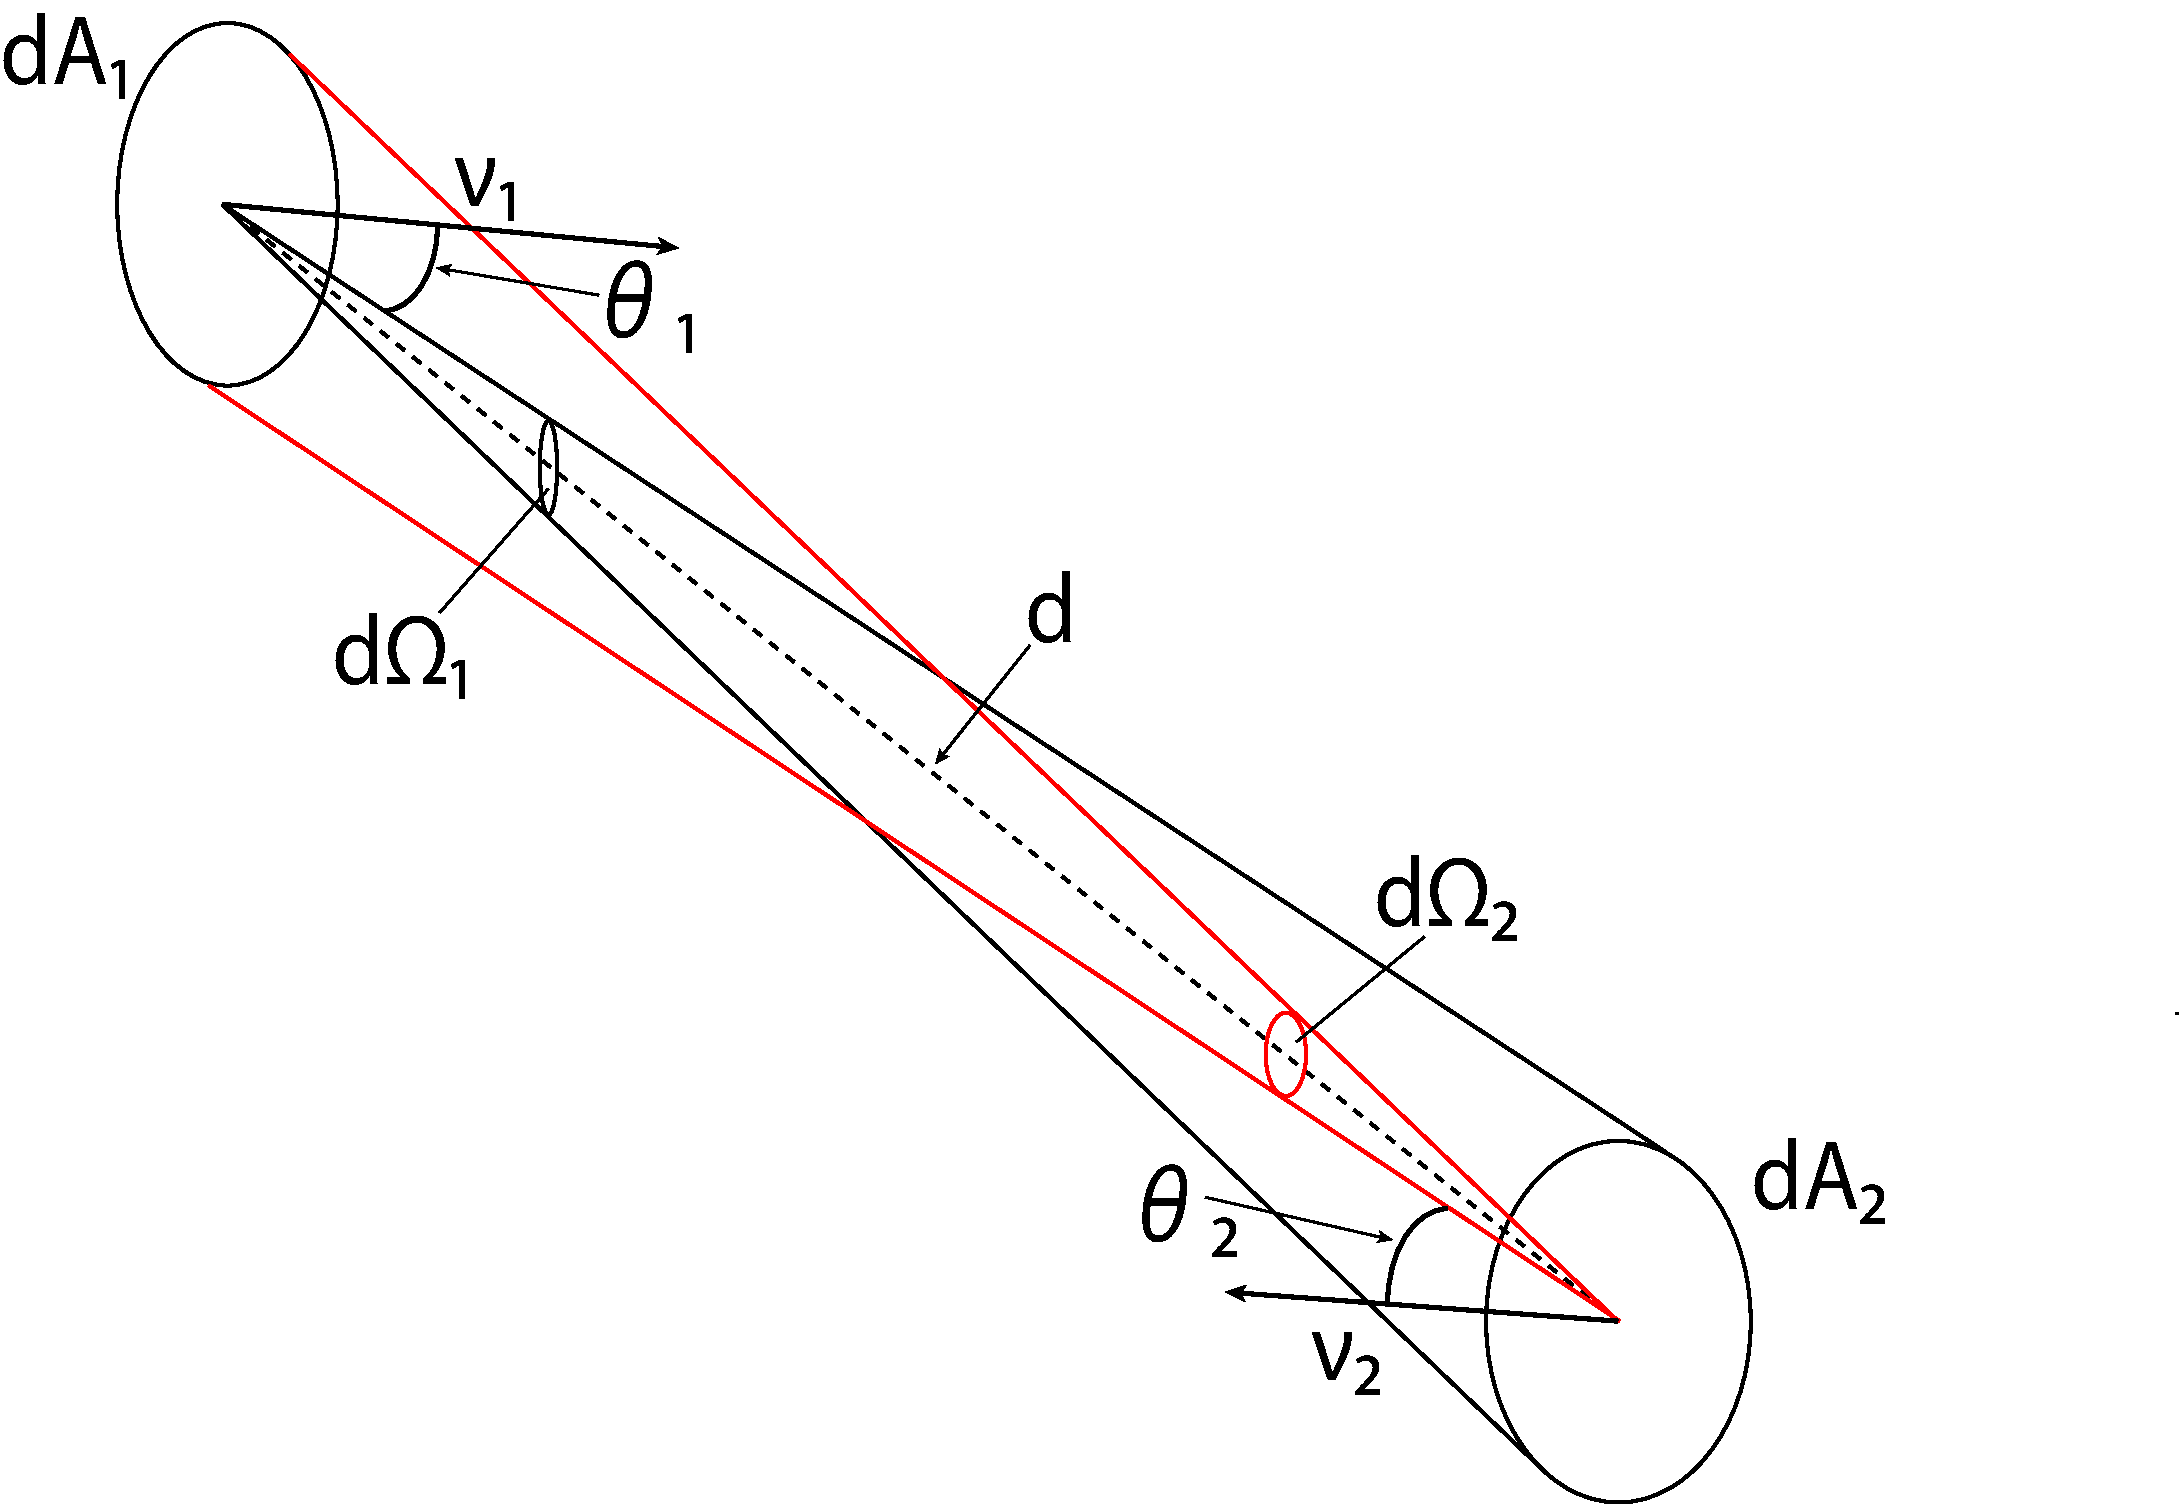
\includegraphics[width=10cm]{areas.pdf}
     \end{center}
     \caption{\footnotesize{$\textrm{d}A_1$ and $\textrm{d}A_2$ are two surfaces with normals $\nu_1$ and $\nu_2$, respectively. Their centers are located at a distance \variabile{d}.
\myangle$_1$ and \myangle$_2$ are the angles made by the central ray with the normals $\nu_1$ and $\nu_2$, respectively.}}
\label{fig:etendue_conservation}
 \end{figure}
Indicating with $\boldsymbol{\nu}_1$ and $\boldsymbol{\nu}_2$ the normals to the surfaces $\textrm{d}A_1$ and $\textrm{d}A_2$, respectively and with \myangle$_1$ and \myangle$_2$ the angles that the central ray forms with $\boldsymbol{\nu}_1$ and $\boldsymbol{\nu}_2$, respectively,
the flux $\textrm{d}\Phi_1$ passing through $\textrm{d}A_2$ coming from $\textrm{d}A_1$ and the corresponding solid angle $\textrm{d}\Omega_1 $ are defined as:
\begin{equation}
\begin{split}
\textrm{d}\Phi_1 &= L \cos\mbox{\myangle}_1 \textrm{d}A_1 \textrm{d}\Omega_1, \\
\textrm{d}\Omega_1 &= \frac{\textrm{d}A_2\cos(\mbox{\myangle}_2)}{\variabile{d}^2}\,.
\end{split}
\end{equation}
Similarly, the flux $\textrm{d}\Phi_2$ passing through $\textrm{d}A_1$ coming from $\textrm{d}A_2$ is equal to:
\begin{equation}\begin{split}
\textrm{d}\Phi_2 &= L \cos\mbox{\myangle}_2 \textrm{d}A_2 \textrm{d}\Omega_2\\
\textrm{d}\Omega_2 &= \frac{\textrm{d}A_1\cos\mbox{\myangle}_1}{\variabile{d}^2}\,.
\end{split}
\end{equation}
Then from Eq. (\ref{etendue}) we obtain the following relations: \begin{equation}
\begin{split}
\textrm{d}U_1 &= n^2 \textrm{d}A_1\cos\mbox{\myangle}_1\textrm{d}\Omega_1= \frac{n^2 \textrm{d}A_1\cos\mbox{\myangle}_1\textrm{d}A_2\cos\mbox{\myangle}_2}{\variabile{d}^2},\\
\textrm{d}U_2 &= n^2 \textrm{d}A_2\cos\mbox{\myangle}_2\textrm{d}\Omega_2= \frac{ n^2 \textrm{d}A_2\cos\mbox{\myangle}_2\textrm{d}A_1\cos\mbox{\myangle}_1	`}{\variabile{d}^2}
\end{split}
\end{equation}
for $\textrm{d}A_1$ and $\textrm{d}A_2$, respectively.
%From equation ($\ref{etendue1}$) and ($\ref{etendue2}$) 
From the previous equations we can conclude that $\textrm{d}U_1=\textrm{d}U_2$ and therefore the \'{e}tendue $\textrm{d}U$ is conserved along a beam of light. 
Since also the flux through the areas $\textrm{d}A_1$ and $\textrm{d}A_2$ is conserved, the following relation holds:
\begin{equation}\label{basicluminance}
L := n \frac{\textrm{d}\Phi}{\textrm{d}U} = constant\,.
\end{equation}
 In the optical systems we will consider in this work, the source and the target are located in the same medium (air) with $n=1$, so the luminance $L$ equals the basic luminance $L^* = L/n$ at the source and the target of the system.\\
\indent In this thesis we consider two-dimensional optical systems. 
 Hence, the definitions of the photometric parameters have to be given in two dimensions. An infinitesimal line segment of length $\textrm{d}\variabile{a}$ that emits a light beam is considered. The central ray of the beam makes an angle \myangle with its normal $\boldsymbol{\nu}$ is considered, see Fig. \ref{}. 
 The two-dimensional illuminance \big(unit $\big[\textrm{lm}/\textrm{m}\big]$\big) denotes the luminous flux falling on an infinitesimal line segment of length $\textrm{d}\variabile{a}$ 
and it is given by:
 \begin{equation}
 E=\frac{\textrm{d}\Phi}{\textrm{d}\variabile{a}}\;.
 \end{equation}
 The luminous intensity \big(unit $\big[\textrm{lm}/\textrm{rad}\big]$\big) is the luminous flux per angle $\textrm{d}\mbox{\myangle}$:
 \begin{equation}
 I=\frac{\textrm{d}\Phi}{\textrm{d}\mbox{\myangle}}\;.
 \end{equation}
 The two-dimensional luminance \big(unit $\big[\textrm{lm}/(\textrm{rad}\; \textrm{m})\big]$\big) is given by:
 \begin{equation}
 L= \frac{\textrm {d}\Phi}{\cos\mbox{\myangle}\,\textrm{d}\variabile{a} \,\textrm{d}\mbox{\myangle}}.
 \end{equation}
 Thus the following relation holds:
 \begin{equation}
 I = L(\vect{x}, \mbox{\myangle})\cos\mbox{\myangle}\,\textrm{d}\variabile{a}\,.
 \end{equation}
 Finally, the \'{e}tendue $\textrm{d}U $ (unit $[\textrm{m}\textrm{rad}]$) in two dimensions is given by:
\begin{equation}\label{etendue2d}
\textrm{d}U = n\cos\mbox{\myangle}\textrm{d}\variabile{a}\,\textrm{d}\mbox{\myangle}.
\end{equation}
In order to determine the light distribution on a certain surface and to compute the photometric variables on that surface, we need to understand how the light emitted from the source propagates. In the field of geometric optics the light propagation is described by light rays.
The propagation of a light ray traveling through  different media is determined by the reflection and refraction law.
In the following we introduce these two laws and we explain the total internal reflection phenomenon.
\section{Reflection and refraction law}\label{sec:reflection}
A light ray is described by a position vector \vect{x} on a surface and a direction vector \vect{t} and can be parameterized by the arc length \variabile{s}.
Light rays travel in a homogeneous medium along straight lines, once they hit a reflective surface their direction changes.
 Denoting with $\vect{t}_\textrm{i}$ the direction of the incident ray and with $\boldsymbol{\nu}$ the unit normal to the surface at the location of incidence, the direction $\vect{t}_\textrm{r}$ of the reflected ray is given by:
 \begin{equation}\label{Reflection}
  \vect{t}_\textrm{r} = \vect{t}_\textrm{i}-2 (\vect{t}_\textrm{i}\boldsymbol{\cdot}\boldsymbol{\nu})\boldsymbol{\nu}\,,
\end{equation}
where the vectors $\vect{t}_\textrm{i}$ and $\boldsymbol{\nu}$ are unit vectors and $\vect{t}_\textrm{i}\boldsymbol{\cdot}\boldsymbol{\nu}$ indicates the scalar product between 
$\vect{t}_\textrm{i}$ and $\boldsymbol{\nu}$. 
From Eq. (\ref{Reflection}) it follows that the vector  $\vect{t}_\textrm{r}$ is a unit vector too, indeed considering the scalar product $(\vect{t}_\textrm{r},\vect{t}_\textrm{r})$ we conclude:
\begin{equation}\label{unit_vector}
\vect{t}_\textrm{r}\boldsymbol{\cdot}\vect{t}_\textrm{r} = \vect{t}_\textrm{i}\boldsymbol{\cdot}\vect{t}_\textrm{i} 
- 4(\vect{t}_\textrm{i}\boldsymbol{\cdot}\boldsymbol{\nu})(\vect{t}_\textrm{i}\boldsymbol{\cdot}\boldsymbol{\nu})+
4(\vect{t}_\textrm{i}\boldsymbol{\cdot}\boldsymbol{\nu})^2(\boldsymbol{\nu}\boldsymbol{\cdot}\boldsymbol{\nu})=1 .
\end{equation} 
The vectors $\vect{t}_\textrm{i}$, $\vect{t}_\textrm{r}$ and $\boldsymbol{\nu}$ live all in the same plane.
Defining the incident angle \myangle$_\textrm{i}$ and the reflective angle \myangle$_\textrm{r}$ such that \myangle$_\textrm{i}$, \myangle$_\textrm{r} \in[0, \pi/2)$.
%\begin{equation}
%\cos{\mbox{\myangle}_\textrm{i}} = -\vect{t}_\textrm{i}\cdot \boldsymbol{\nu} \qquad \mbox{and} \qquad \cos{\mbox{\myangle}_\textrm{r}} = \vect{t}_\textrm{r} \cdot\boldsymbol{\nu}\,,
%\end{equation}
the reflection law states that \myangle$_\textrm{i}=$ \myangle$_\textrm{r}$, see Fig. \ref{fig:Snell}.
\begin{figure}[h]
 \label{fig:Snell}
     \begin{center}
     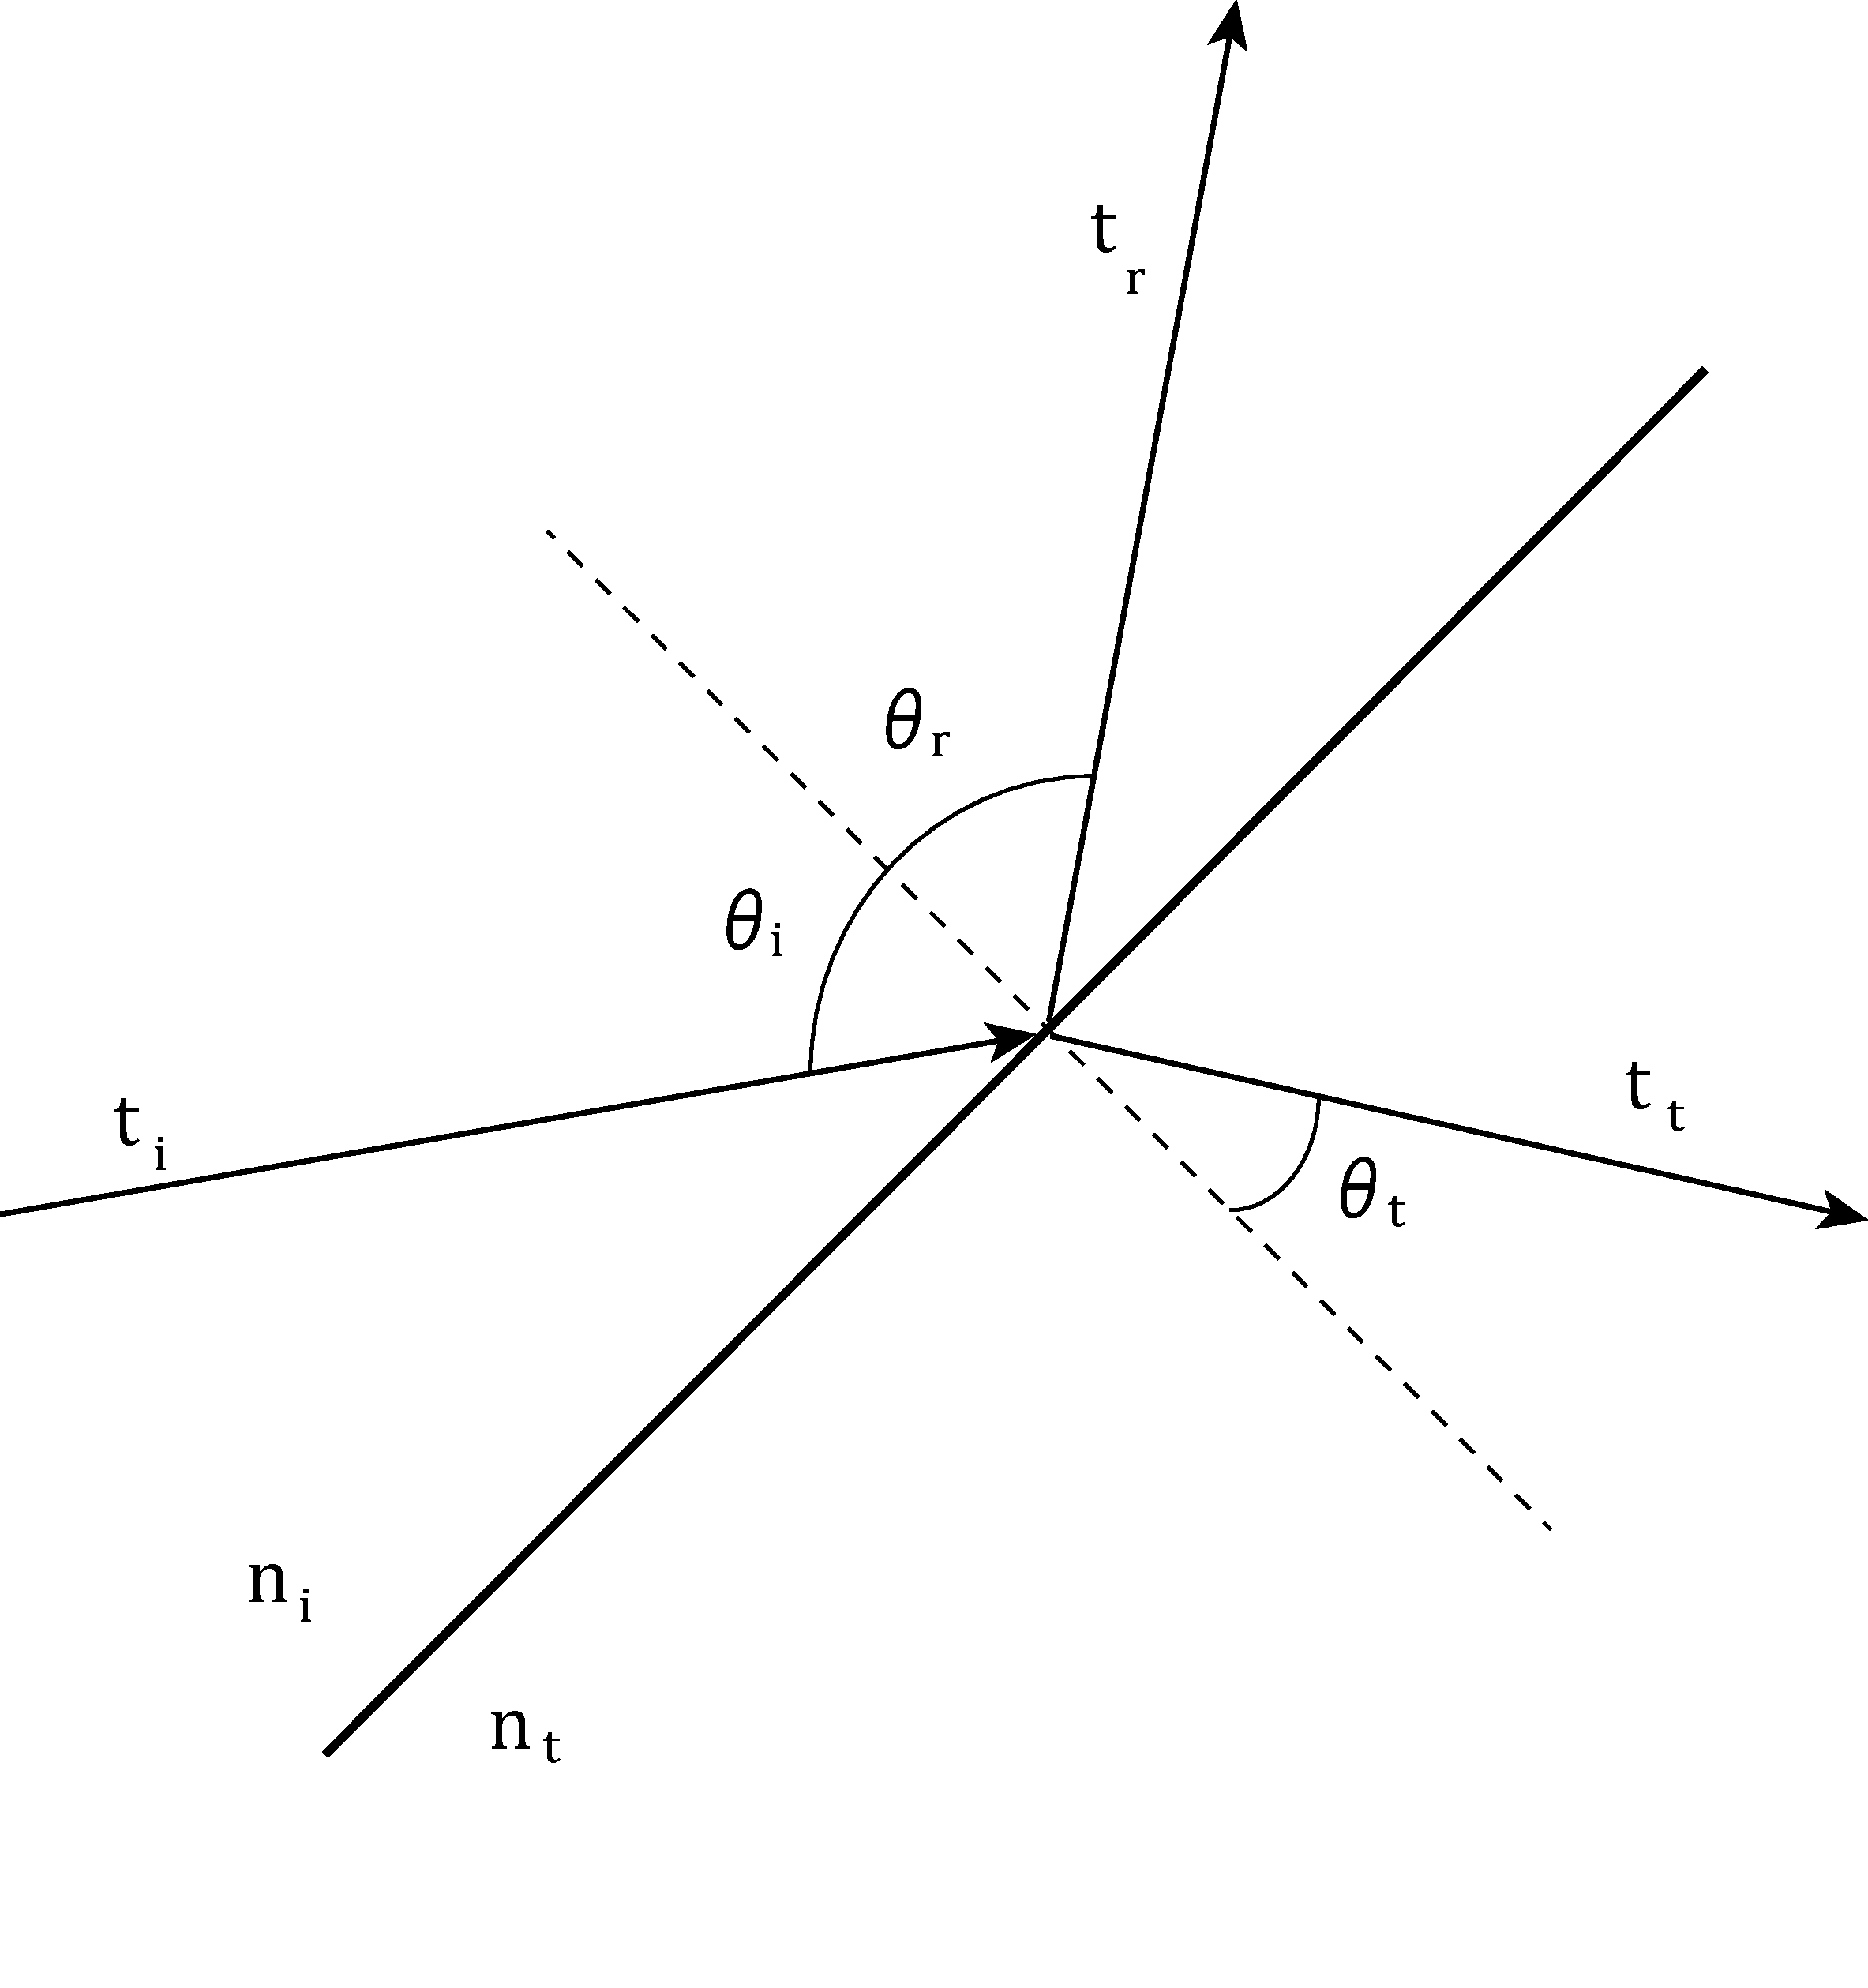
\includegraphics[width=8cm]{reflection}
     \end{center}
     \caption{Propagation of a ray through two different media with index of refraction $n_\textrm{i}$ and $n_\textrm{t}$.}% \bolsymbol{$\nu$} is the normal to the surface $A$ that the incident ray hits.
%$\vect{t}_i$, $\vect{t}_r$ and $\vect{t}_t$ are the direction vectors of the incident, reflected and refracted (or transmitted) ray, respectively. }}
%\myangle$_{i}$, \myangle$_{r}$ and \myangle$_{t}$ are the angles between \bolsymbol{$\nu$} and the incident, reflected and transmitted ray, respectively.}}
\label{fig:Snell}
 \end{figure}
\\ When a ray propagates through two different media, its direction changes according to the law of refraction. 
Indicating with $n_\textrm{i}$ the index of refraction of the medium in which the incident ray travels and with 
$n_\textrm{t}$ the index of refraction of the medium of the transmitted ray, the direction $\vect{t}_\textrm{t}$ of the transmitted ray is given by:
\begin{equation}\label{Refraction}
\vect{t}_\textrm{t} = n_{\textrm{i},\textrm{t}}\,\vect{t}_\textrm{i}+
\Big[\sqrt{1-n_{\textrm{i}\boldsymbol{\cdot}\textrm{t}}^2+
n_{\textrm{i},\textrm{t}}^2(\boldsymbol{\nu}\boldsymbol{\cdot}\vect{t}_\textrm{i})^2}
-n_{\textrm{i},\textrm{t}}(\boldsymbol{\nu}\boldsymbol{\cdot}\vect{t}_\textrm{i}) \Big]\boldsymbol{\nu}\,,
\end{equation}
where $n_{\textrm{i},\textrm{t}}=n_\textrm{i}/n_\textrm{t}$, \cite{chaves2015introduction}.
 Note that in Eq. (\ref{Reflection}) the direction of the normal $\boldsymbol{\nu}$ to the surface is not relevant for the computation of the direction of the reflective ray, since:
\begin{equation}
\vect{t}_\textrm{r} = \vect{t}_\textrm{i}-2(\vect{t}_\textrm{i}\boldsymbol{\cdot}\boldsymbol{\nu})\boldsymbol{\nu}= \vect{t}_\textrm{i}-2(\vect{t}_\textrm{i}\boldsymbol{\cdot}-\boldsymbol{\nu})(-\boldsymbol{\nu}) ,
\end{equation}
however, this is not the case for Eq. (\ref{Refraction}), therefore in the latter case we need to specify the direction of $\boldsymbol{\nu}$ which is usually chosen in such a way that the angle that it forms with the incident ray $\vect{t}_\textrm{i}$ is smaller than or equal to $\pi/2$. Hence, if $(\vect{t}_\textrm{i}, \boldsymbol{\nu})\leq0$ the normal $\boldsymbol{\nu}$ directed inside the same medium in which travels the incident ray is taken as in Fig. \ref{fig:Snell}, 
otherwise the normal $-\boldsymbol{\nu}$ directed inside the same medium in which the transmitted ray will travel has to be considered.
\\\indent
Eq. (\ref{Refraction}) is only valid for 
\begin{equation}\label{tir}
1-n_{\textrm{i},\textrm{t}}^2+n_{\textrm{i},\textrm{t}}^2(\boldsymbol{\nu}\boldsymbol{\cdot}\vect{t}_\textrm{i})^2\geq 0 
\end{equation} which implies that
\begin{equation}
\frac{n_\textrm{t}}{n_\textrm{i}}\geq \sqrt{1-(\boldsymbol{\nu}\boldsymbol{\cdot}\vect{t}_\textrm{i})^2}
\end{equation}
from which we obtain:
\begin{equation}
 %n_\textrm{t}\geq n_\textrm{i}\sqrt{1-\cos^2\mbox{\myangle}_\textrm{i}}= 
 n_\textrm{t}\geq n_\textrm{i} \sin\mbox{\myangle}_\textrm{i}\,.
\end{equation}
 The angle $\mbox{\myangle}_{\textrm{c}}$ for which the equality holds is
\begin{equation}\label{critical}
\mbox{\myangle}_{\textrm{c}} = \arcsin\Big(\frac{n_\textrm{t}}{n_\textrm{i}}\Big)
\end{equation} and it is called the critical angle, \cite{chaves2015introduction}.
%Note that the condition $\frac{n_t}{n_i}<1$ is verified as in this case $\sin(\mbox{\myangle}_\textrm{i})<1$.
When the incident angle \myangle$_{\textrm{i}}$ is exactly equal to the critical angle \myangle$_{\textrm{c}}$, the square root in Eq. (\ref{Refraction}) is zero and the inner product $(\vect{t}_\textrm{t},\boldsymbol{\nu})=0$, hence the transmitted ray propagates parallel to the refractive surface. 
When \myangle$_{\textrm{i}}>\mbox{\myangle}_{\textrm{c}}$ the light ray is no longer refracted but is only reflected by the surface. This phenomenon is called total internal reflection (TIR). When TIR occurs, $100\%$ of light is reflected and there is no loss of energy. Therefore, optical systems designed such that rays are reflected by TIR are very efficient. Lght that hits an ordinary refractive surface can be reflected and refracted. The energy that is reflected and refracted is determined by the Fresnel's coefficients.
In the next paragraph an overview of the Fresnel coefficients is given.

\section{Fresnel's equations}\label{sec:fresnel}
In order to derive Fresnel's equations we need to describe light as an electromagnetic wave. 
It is therefore useful to study the light propagation from the perspective of electromagnetic theory which gives information about the incident, reflected and transmitted radiant flux density that are denoted with $E_i$, $E_r$ and $E_t$, respectively.  
Any component of the electric field $\boldsymbol{\mathcal{E}}$ can be written as
\begin{equation}\label{electric_field}
\boldsymbol{\mathcal{E}}(\vect{x}, \mytime) = \boldsymbol{\mathcal{E}}_0(\vect{x} )e^{i( \vect{k}\boldsymbol{\cdot}\vect{x}-\omega \mytime )}
\end{equation}
where \vect{x} is the position vector and $T$ is the time. The amplitude $\boldsymbol{\mathcal{E}}_0(\vect{x})$ is constant in time and $\omega = \frac{c k}{n}$ is the value of the angular frequency with $c$ the velocity of light and $n$ the index of refraction in which the wave is traveling, which is the ratio of the speed of light $c$ in vacuum and the speed of light $v$ in the material. Note that the angular frequency can be also written as $\omega = vk$, in particular when a wave travels in vacuum $n=1$ and $\omega=ck$. The vector \vect{k} has the same direction of the wave and its absolute value 
$|\vect{k}| = k = \frac{2\pi}{\lambda}$ is the wave number in vacuum, with $\lambda$ the wavelength. Similarly, the magnetic field has the form:
\begin{equation}
\boldsymbol{\mathcal{B}}(\vect{x}, \mytime) = \boldsymbol{\mathcal{B}}_0(\vect{x}) e^{i( \vect{k}\boldsymbol{\cdot} \vect{x}-\omega \mytime )}\,.
\end{equation}
Light can be seen as an electromagnetic wave, that is an oscillating electric field $\boldsymbol{\mathcal{E}}$ and an oscillating magnetic filed $\boldsymbol{\mathcal{B}}$ which propagates  always perpendicular to $\boldsymbol{\mathcal{E}}$. 
In order to derive the Fresnel's coefficients the polarization of light must to be taken into account. 
Those coefficients are obtained considering the Maxwell's equations and the boundary conditions due to the conservation of energy.
The details of Fresnel's equations are widely explained in the literature. 
In the following we provide Fresnel coefficients and we briefly explain their physical interpretation. We refer the reader to \cite{born2013principles, hecht1998hecht} for more details. 
Fresnel's coefficients can also be derived using a different approach that does not involve Maxwell's equations, this method is explained in \cite{feynman2011feynman}. 
By convention, we refer to the light's polarization as the direction of the electric field $\boldsymbol{\mathcal{E}}$, \cite{feynman1964feynman} with respect to the incident plane that is defined by the incident and reflected rays as is shown in Fig. \ref{}. The electric field can propagate in any direction, Fresnel's equations are derived considering two particular cases of light's polarization. 
\begin{enumerate}
\item $\boldsymbol{\mathcal{E}}$ is perpendicular to the plane of incidence (see Fig. \ref{}). In this case  light is said to be $s$-polarized.
\item $\boldsymbol{\mathcal{E}}$ is parallel to the plane of incidence (see Fig. \ref{}). In this case light is said to be $p$-polarized.
\end{enumerate}
Energy conservation gives the boundary conditions of the electromagnetic field at the plane of the interface (which is perpendicular to the incident plane). \\ 
\indent In case of $s$-polarized light the tangential components of $\boldsymbol{\mathcal{E}}$ and $\boldsymbol{\mathcal{B}}/\mu$ across the boundary between the two different media must be continuous. The continuity of the tangential component of $\boldsymbol{\mathcal{E}}$ leads to:
\begin{equation}\label{Econservation}
|\boldsymbol{\mathcal{E}}_{0\textrm{i}}|+|\boldsymbol{\mathcal{E}}_{0\textrm{r}}|= |\boldsymbol{\mathcal{E}}_{0\textrm{t}}|
\end{equation} 
%where we have indicated with $\mathcal{E}_{0\textrm{i}}$, $\mathcal{E}_{0\textrm{r}}$ and $\mathcal{E}_{0\textrm{t}}$
%the magnitudes of $\boldsymbol{\mathcal{E}}_{0\textrm{i}}$, $\boldsymbol{\mathcal{E}}_{0\textrm{r}}$ and $\boldsymbol{\mathcal{E}}_{0\textrm{t}}$, respectively.
while the continuity of the tangential component of $\boldsymbol{\mathcal{B}}/\mu$ gives:
\begin{equation}\label{Bconservation}
-\frac{|\boldsymbol{\mathcal{B}}_{\textrm{i}}|}{\mu_\textrm{i}}\cos\mbox{\myangle}_{\textrm{i}}+\frac{|\boldsymbol{\mathcal{B}}_{\textrm{r}}|}{\mu_\textrm{r}}\cos\mbox{\myangle}_{\textrm{r}} = 
-\frac{|\boldsymbol{\mathcal{B}}_{\textrm{t}}|}{\mu_\textrm{t}}\cos\mbox{\myangle}_{\textrm{t}}
\end{equation}
%where we have indicated with $\mathcal{B}_{\textrm{i}}$, $\mathcal{B}_{\textrm{r}}$ and $\mathcal{B}_{\textrm{t}}$
%the absolute values of $\boldsymbol{\mathcal{B}}_{\textrm{i}}$,$\boldsymbol{\mathcal{B}}_{\textrm{r}}$ and $\boldsymbol{\mathcal{B}}_{\textrm{t}}$, respectively.
Since $\boldsymbol{\mathcal{B}} = \boldsymbol{\mathcal{E}}/v$, Eq. (\ref{Bconservation}) can be written as 
\begin{equation}
\frac{1}{\mu_{\textrm{i}}v_{\textrm{i}}}(|\boldsymbol{\mathcal{E}}_{\textrm{i}}|-|\boldsymbol{\mathcal{E}}_{\textrm{r}}|)\cos\mbox{\myangle}_{\textrm{i}} = \frac{1}{\mu_{\textrm{t}}v_{\textrm{t}}}|\boldsymbol{\mathcal{E}}_{\textrm{t}}|\cos\mbox{\myangle}_{\textrm{t}}
\end{equation}
where we employed the fact that $v_{\textrm{i}}= v_{\textrm{r}}$, and $\mbox{\myangle}_{\textrm{i}}= \mbox{\myangle}_{\textrm{r}}$. 
Using Eq. (\ref{electric_field}) and $n = c/v$, the previous equation becomes:
\begin{equation}
\frac{n_{\textrm{i}}}{\mu_{\textrm{i}}}(|\boldsymbol{\mathcal{E}}_{0\textrm{i}}|-|\boldsymbol{\mathcal{E}}_{0\textrm{r}}|)\cos\mbox{\myangle}_{\textrm{i}} = \frac{n_{\textrm{t}}}{\mu_{\textrm{i}}}|\boldsymbol{\mathcal{E}}_{0\textrm{t}}|\cos\mbox{\myangle}_{\textrm{t}}
\end{equation}
Finally,  assuming that $\mu_{\textrm{i}}=\mu_{\textrm{t}}=\mu_{0}$ and employing Eq. (\ref{Econservation}) we obtain:
\begin{equation} \label{Fresnel_perpendicular}
\begin{split}
r_{s} & =\frac{|\boldsymbol{\mathcal{E}}_{0 \textrm{r}}|_{s}}{|\boldsymbol{\mathcal{E}}_{0\textrm{i}}|_s} = 
\frac{n_\textrm{i}\cos\mbox{\myangle}_\textrm{i}-n_\textrm{t} \cos\mbox{\myangle}_\textrm{t}}{n_\textrm{i}
\cos\mbox{\myangle}_\textrm{i}+n_\textrm{t}\cos\mbox{\myangle}_\textrm{t}},\\
t_{s} & = \frac{|\boldsymbol{\mathcal{E}}_{0 \textrm{t}}|_s}{|\boldsymbol{\mathcal{E}}_{0\textrm{i}}|_s} 
=\frac{2n_\textrm{i}\cos\mbox{\myangle}_\textrm{i}}{n_\textrm{i}\cos\mbox{\myangle}_\textrm{i}+n_\textrm{t}\cos\mbox{\myangle}_\textrm{t}}.\\
\end{split}
\end{equation}
The coefficients $r_s$ and $t_s$ are amplitude coefficients for the reflected and transmitted light.
They are the perpendicular components of $r$ and $t$ for $s$-polarized light.
Using Snell's law, that is $n_{\textrm{i}}\sin\mbox{\myangle}_{\textrm{i}} = n_{\textrm{t}}\sin\mbox{\myangle}_{\textrm{t}}$, the relations for $r_s$ and $t_s$ are simplified as follows:
\begin{equation} \label{simple_Fresnel}
\begin{split}
r_{s} & = -\frac{\sin(\mbox{\myangle}_i-\mbox{\myangle}_t)}{\sin(\mbox{\myangle}_i+\mbox{\myangle}_t)},\\
t_{s} & = -\frac{2\sin \mbox{\myangle}_t \cos \mbox{\myangle}_i}{\sin(\mbox{\myangle}_i+\mbox{\myangle}_t)}\,.
\end{split}
\end{equation}
\indent A similar argument for the $p$-polarized light leads to the calculation of the parallel components $r_p$ and $t_p$ of $r$ and $t$. 
In case $\boldsymbol{\mathcal{E}}$ is parallel to the plane of incidence the amplitude coefficients are:
\begin{equation}\label{Fresnel_parallel}
\begin{split}
r_{p} & = \frac{n_t\cos\mbox{\myangle}_i-n_i \cos\mbox{\myangle}_t}{n_i \cos\mbox{\myangle}_t+n_t\cos\mbox{\myangle}_i},\\
t_{p} & =  \frac{2n_i\cos\mbox{\myangle}_i}{n_i\cos\mbox{\myangle}_t+n_t\cos\mbox{\myangle}_i}\,,
\end{split}
\end{equation}
and their simplified relations are:
\begin{equation} \label{simple_Fresnel}
\begin{split}
r_{p} & =  \frac{\tan(\mbox{\myangle}_i-\mbox{\myangle}_t)}{\mbox{\myangle}_i+\mbox{\myangle}_t},\\
t_{p} & = \frac{2\sin \mbox{\myangle}_t \cos \mbox{\myangle}_i}{\sin(\mbox{\myangle}_i+\mbox{\myangle}_t)\cos(\mbox{\myangle}_i- \mbox{\myangle}_t)}.
\end{split}
\end{equation}
Furthermore, it can be checked that
 \begin{equation}
\begin{split}
t_s-r_s &= 1, \\
t_p+r_p &=  1.
\end{split}
\end{equation}
The amplitude coefficients are shown in Fig. \ref{fig:coefficients} for the case in which light travels from a less dense to a more dense medium ($n_i<n_t$), that is external reflection. 
In Fig. \ref{fig:coefficients2} the reflection coefficients are shown for the case in which $n_i>n_t$, that is internal reflection. Note from Fig. \ref{fig:coefficients} that $r_p$ approaches to $0$ when \myangle$_i$ approaches to \myangle$_p$ and it gradually decreases reaching $-1$ for an incident angle \myangle$_i=90^\circ$. The angle \myangle$_p$ is called Brewster's angle or polarization angle as only the component perpendicular to the incident plane is reflected at that angle and therefore light is perfectly polarized. Similarly, Fig. \ref{fig:coefficients2} shows that $r_p=0$ for \myangle$_i= $ \myangle$_{p\prime}$. It can be show that \myangle$_p+ $\myangle$_{p\prime}= 90^\circ$. Both $r_p$ and $r_s$ reach $1$ when \myangle$_i= $ \myangle$_c$. \myangle$_c$ is called the critical angle. Light that hits the incident plane with an incident angle equal to or greater than the critical angle is totally reflected back and no transmitted light is observed. This phenomenon is called total internal reflection. 
\begin{figure}[h]
  \begin{minipage}[h]{0.4\textwidth}
    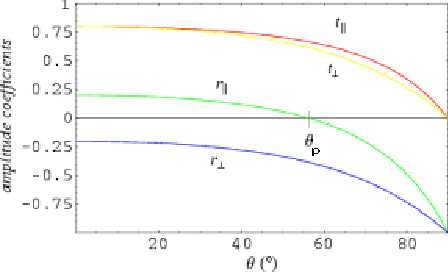
\includegraphics[width=\textwidth]{amplitude_coefficients2.pdf}
    \caption{Amplitude coefficients of reflection and transmission as a function of the incident angle \myangle$_i$  in the case of external reflection, i.e. $n_t<n_i$
($n_t = 1$ and $n_i=1.5$). \myangle$_p$ is the polarization angle, \cite{hecht1998hecht}.}
    \label{fig:coefficients}
  \end{minipage} \hspace{2.5cm}
  \begin{minipage}[h]{0.4\textwidth}
    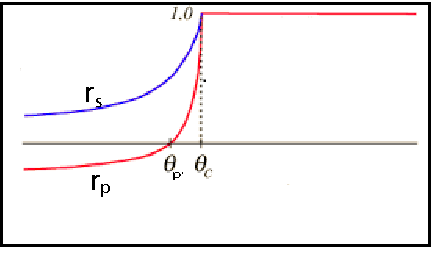
\includegraphics[width=\textwidth]{rprs.pdf}
    \caption{Reflection coefficients as a function of the incident angle \myangle$_i$ in the case of internal reflection, i.e. $n_t>n_i$
($n_t = 1.5$ and $n_i=1$). \myangle$_{p\prime}$ is the polarization angle and \myangle$_c$ is the critical angle, \cite{hecht1998hecht}.}
   \label{fig:coefficients2}
 \end{minipage}
\end{figure}\\
\indent The  we introduce the Poynting vector \vect{P} that defines the energy flux of an electromagnetic field. 
It is measured in $[\textrm{W}/\textrm{m}^2]$, and it is given by:
\begin{equation}
\vect{P} = \frac{1}{\mu}\Big(\boldsymbol{\mathcal{E}}\boldsymbol{\times} \boldsymbol{\mathcal{B}}\Big),
\end{equation}
where $\mu = \frac{1}{\varepsilon v^2}$ is the permeability and $\varepsilon$ the permittivity of the medium.
 In the following, the parameters for vacuum are indicated with the subscript $0$. All quantities defined in the media of the incident, reflective and transmitted light are indicated with the subscripts \textrm{i}, \textrm{r} and \textrm{t}, respectively. Optical rays are perpendicular to the wave front of an electromagnetic wave and parallel to the Poynting vector, \cite{jones2015optical}.
The irradiance $E$ is defined as the average energy that crosses in unit time a unit area $A$ perpedicular to the direction of the energy flow.
Therefore, defining the average of the vector \vect{P} over the time as:
\begin{equation}
\langle \vect{P} \rangle_T = \frac{1}{T}\int_0^T \vect{P}\textrm{d}T
\end{equation}
we can write the irradiance $E$ as:
\begin{equation}
\vect{E} = \langle\vect{P}\rangle_{\mytime} = v\varepsilon|\boldsymbol{\mathcal{E}}|^2 \,.
\end{equation}
Considering a beam of light that hits a surface such that an area $A$ is illuminated, the incident, reflected and transmitted beams are 
$\vect{E}_\textrm{
i} A\cos\mbox{\myangle}_\textrm{i}$ $\vect{E}_\textrm{r} A\cos\mbox{\myangle}_\textrm{r}$ and 
$\vect{E}_\textrm{t} A\cos\mbox{\myangle}_\textrm{t}$, respectively as is shown in Fig. \ref{}
The reflectance $\mathcal{R}$ is the ratio of the reflected power to the incident power:
\begin{equation}\label{reflectance}
\mathcal{R} = \frac{|\vect{E}_\textrm{r}|\cos\mbox{\myangle}_r}{|\vect{E}_\textrm{i}|\cos\mbox{\myangle}_\textrm{i}} = \frac{|\boldsymbol{\mathcal{E}}_{0 \textrm{r}}|^2}{|\boldsymbol{\mathcal{E}}_{0 \textrm{i}}|^2} = r^2
\end{equation}
where the second equality holds because $v_{\textrm{i}}= v_{\textrm{t}}$, $\varepsilon_{\textrm{i}} = \varepsilon_{\textrm{t}}$ and $\mbox{\myangle}_{\textrm{i}} = \mbox{\myangle}_{\textrm{t}}$.
Similarly, the transmittance $\mathcal{T}$ is the ratio between the transmitted to the incident power:
\begin{equation}\label{transmittance}
\mathcal{T} = \frac{|\vect{E}_\textrm{t}| \cos\mbox{\myangle}_\textrm{t}}{|\vect{E}_\textrm{r}|\cos\mbox{\myangle}_\textrm{r}} = \frac{n_\textrm{t} \cos\mbox{\myangle}_\textrm{t}}{n_\textrm{t} \cos\mbox{\myangle}_\textrm{i}}\frac{|\boldsymbol{\mathcal{E}}_{0 \textrm{t}}|^2}{\boldsymbol{|\mathcal{E}}_{0 \textrm{i}}|^2} = \frac{n_\textrm{t} \cos\mbox{\myangle}_\textrm{t}}{n_\textrm{t} \cos\mbox{\myangle}_\textrm{i}} t^2\,.
\end{equation}
Employing total energy conservation, that is:
\begin{equation}
\vect{E}_\textrm{i} A\cos\mbox{\myangle}_\textrm{i} = \vect{E}_\textrm{r} A\cos\mbox{\myangle}_\textrm{r}+\vect{E}_\textrm{t} A\cos\mbox{\myangle}_\textrm{t},
\end{equation}
we can easily prove that:
\begin{equation}
\mathcal{R}+\mathcal{T}=1\,.
\end{equation}
 The parallel and perpendicular components of $\mathcal{R}$ and $\mathcal{T}$ are:
\begin{equation}\label{Fresnel_pands}
\begin{split}
\mathcal{R}_p& =  {r_p^2},\\
\mathcal{T}_p &=  \frac{n_t \cos\mbox{\myangle}_t}{n_t \cos\mbox{\myangle}_i}t_p^2,\\
\mathcal{R}_s &=  r_s^2,\\
\mathcal{T}_s &= \frac{n_t \cos\mbox{\myangle}_t}{n_t \cos\mbox{\myangle}_i}t_s^2.\\
\end{split}
\end{equation}
it can be show that
\begin{equation}
\begin{split}
\mathcal{R}_s+\mathcal{R}_p &= 1,\\
\mathcal{T}_s+\mathcal{T}_p &=1\,.
\end{split}
\end{equation}
For normal incidence, i.e. \myangle$_i = 0$, there is no polarization and Eqs. (\ref{Fresnel_pands}) lead to:
\begin{equation}
\begin{split}
\mathcal{R} &= \mathcal{R}_p = \mathcal{R}_s = \Bigg(\frac{n_i-n_t}{n_t+n_i}\Bigg)^2, \\
\mathcal{T} &= \mathcal{T}_p = \mathcal{T}_s = \frac{4n_i n_t}{(n_t+n_i)^2}\,.
\end{split}
\end{equation}
\indent In two dimensions light hits lines instead of surfaces. Therefore only the plane of incidence is defined and it has no sense to consider separately the parallel and the perpendicular polarization. The amount of reflected and transmitted light is given by the reflectance $\mathcal{R}$ and transmittance $\mathcal{T}$ which are defined as:
\begin{equation}\begin{split}
\mathcal{R} &= \frac{\mathcal{R}_p+ \mathcal{R}_s}{2},\\
\mathcal{T} &= \frac{\mathcal{T}_p+ \mathcal{T}_s}{2}, 
\end{split}
\end{equation}
 where $\mathcal{R}_p$, $\mathcal{R}_s$, $\mathcal{T}_p$ and $\mathcal{T}_s$ are given in Eqs. (\ref{Fresnel_pands}). \\
\indent With this overview we conclude this chapter. The notions given in Section \ref{sec:photometry} will be used in the entire thesis as our goal is to study the distribution of light at the target of some optical systems. In particular we will focus on the computation of the output intensity distribution. The reflection and refraction laws explained in Section \ref{sec:reflection}are needed to determine how the optical system changes the ray's direction every time that it hits a surfaces (or a line in the two-dimensional case). In Chapters \ref{chap:raytracing},\ref{chap:PS}, \ref{chap:triangulation}, \ref{chap:raymapping1} and \ref{chap:raymapping2} only systems where the reflection and refraction laws play a role are considered. Finally, in the last chapter of this work systems where also Fresnel reflection are taken into account.




























